\documentclass[main.tex]{subfiles}
\begin{document}

\chapter{Preliminary notions}
For this chapter we loosely refer to~\cite{abate2011geometria} and~\cite{nakahara2002}. All manifolds in these notes are assumed to be Hausdorff and second-countable.

\section{Smooth manifolds}
A smooth manifold is a topological space which locally looks like an Euclidean space $\R^n$. To fix notation for the rest of the notes, we work out the precise definition behind this intuition.

\begin{definition}
	A \textbf{chart} on a topological space $M$ is a pair $(U, \phi)$ where $U$ is an open subset of $M$ and $\phi$ is an homeomorphism\footnote{An \textbf{homeomorphism} is an isomorphism of topological spaces, hence a continuous map whose inverse is again continuous.} from $U$ to an open set $V \subseteq \R^n$, for suitable $n$.
\end{definition}

A chart then brings the coordinates of $\R^n$ onto $M$:

\begin{figure}[H]
	\centering
	\begin{tikzpicture}
		\node (image) at (0,0) {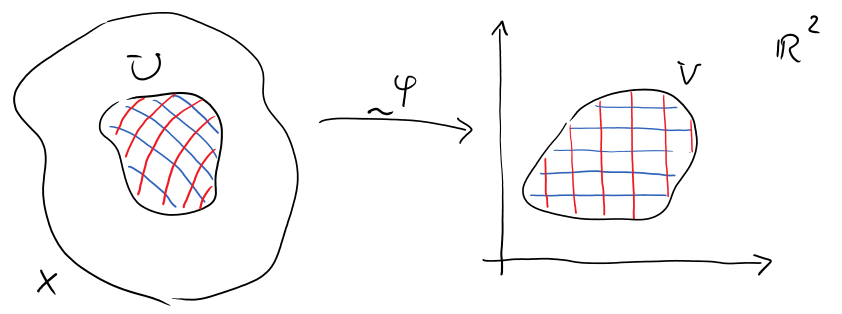
\includegraphics[width=.65\textwidth]{figures/chart.png}};
	\end{tikzpicture}
\end{figure}

Indeed, more often we'll not address directly the map $\phi$ but its components $\phi = (x^1, \ldots, x^n)$. We'll usually say something like: let $(x^1, \ldots, x^n)$ be coordinates around\footnote{Usually this will imply, additionally, that $\phi(p) = 0$, so that we are taken $\im \phi$ to be a neighbourhood of the origin.} $p \in M$. This means we do not give much importance to $U$ either, as long as we know it contains our point of interest.

Finally, notice that when two charts $(U_1, \phi_1)$ and $(U_2, \phi_2)$ overlap, then they are automatically ``compatible'' on their intersection, since $\phi_2 \circ \phi_1^{-1} : \phi_1(U_1 \cap U_2) \isoto \phi_2(U_1 \cap U_2)$ defines an homeomorphism on them. These maps are called \textbf{transition maps} and sew together the different local descriptions of the space $M$.

\begin{definition}
	A \textbf{smooth manifold} is a topological space $M$ together with a \textbf{smooth atlas}, i.e. a collection $\mathcal A = \{(U_i, \phi_i)\}_{i \in I}$ of charts such that all the transition maps are $\Cinfty$-diffeomorphisms\footnote{Hence homeomorphisms which are differentiable infinitely many times.}.
\end{definition}

\begin{remark}
	We stress the last word of the definition: as any two overlapping charts are ``topologically comaptible'', the smoothness of the manifold is ensued by the differentiability of the transition maps.
\end{remark}

We conclude this brief introduction by noting that we rarely give an explicti atlas along with our manifolds. The reason is twofold:
\begin{enumerate}
	\item for most spaces (e.g. spheres, tori, projective spaces), geometers worked out their construction in terms of an atlas once, and then it is understood we are using that;
	\item we always assume the atlas to be \textbf{maximal}, that is, to contain every possible compatible chart (with a given starting set): as such a collection is clearly very large, it is impossible to give one explicitly.
\end{enumerate}

\section{Vector bundles}
On a smooth manifold we are interested in studying so-called differential objects: vectors and forms, as well as smooth functions supported on the manifold.

\begin{definition}
	A \textbf{map of smooth manifolds} $F:M \to N$ is a map from the manifold $M$ to the manifold $N$ which is locally represented by a differentiable function, i.e. for every $p \in M$, there exist a chart $(U, \phi)$ around $p$ and a chart $(V, \psi)$ around $F(p)$ such that $\psi \circ F \circ \phi^{-1}$ is a differentiable function in the usual sense.
\end{definition}

The space of differentiable maps from $M$ to $\R$ is denoted by $\Cinfty(M)$. It clearly is an $\R$-algebra, i.e. a ring whose addition makes it into an $\R$-module.

\begin{definition}
	A \textbf{vector bundle} on a smooth manifold $M$ is a map $\pi : E \to M$ from a smooth manifold $E$ called the \textbf{total space} to the manifold $M$ called the \textbf{base space} such that
	\begin{enumerate}
		\item $\pi^{-1}(p)$ is a vector space for any $p$,
		\item for each $p$, there is an open neighbourhood $U$ of $p$ and a diffeomorphism $\chi :\pi^{-1}(U) \isoto U \times \pi^{-1}(p)$ which is fiberwise an isomorphism of vector spaces and makes the following commute:
		\begin{diagram}
			\pi^{-1}(U) \arrow{d}{\pi} \arrow{r}{\chi} \& U \times \pi^{-1}(p) \arrow{dl}{\pr_1}\\
			U
		\end{diagram}
	\end{enumerate}
\end{definition}

Intuitively, a vector bundle is a smooth assignment of vector spaces to each point of a manifold. A consequence of this is that every fiber $\pi^{-1}(p)$ has the same dimension $r$, called the \textbf{rank} of the bundle.

\begin{definition}
	A \textbf{section} of a vector bundle $\pi : E \to M$ is any map $s : M \supseteq U \to E$ which is a left inverse of $\pi$ on $U$, i.e. \begin{eqalign}
		\pi \circ s = \id_U.
	\end{eqalign}
	If $U=M$, the section is said to be \textbf{global}.
\end{definition}

A section of a vector bundle can be more easily depicted as a smooth assignment of vectors of $E$, where the vector at $p \in M$ is taken from the fiber there.

The most important vector bundle in differential geometry is the \textbf{tangent bundle} $TM$. Its construction is somewhat technical so we refer to \cite{abate2011geometria}, but intuitively it is the vector bundle whose fiber at $p \in M$ is the space of tangent vectors at $p$, suitably defined. Global sections of $TM$ are called \textbf{vector fields} and the totality of them is denoted by $\fields(M)$.

Along with $TM$, we get the \textbf{cotangent bundle} $T^*M$, whose fibers are dual to those of $TM$. Global sections of $T^*M$ are called \textbf{differential $1$-forms} and the totality of them is denoted by $\Omega^1(M)$.

Finally, through fiberwise tensoring we get a \textbf{tensor bundle} $T^p_q M$ for each $p, q \in \N$. Global sections of $T^h_k$ are called \textbf{$h$-covariant, $k$-contravariant tensors}, or simply \textbf{tensors of type $(h, k)$}. Clearly $T^1 M = TM$ and $T_1 M = T^* M$. When after tensoring, we look at the skew-symmetric part of the tensors, we get an algebra called the \textbf{external algebra} of $M$. The product is denoted by $\wedge$, and is defined as
\begin{eqalign}
	\xi_1 \wedge \ldots \wedge \xi_q = \sum_{\sigma \in S_q} (-1)^{\sign \sigma} \xi_{\sigma(1)} \tens \ldots \tens \xi_{\sigma(q)}, \quad \forall \xi_1, \ldots, \xi_q \in T^*M.
\end{eqalign}
Skew-symmetric $k$-contravariant tensors are more commonly referred to as \textbf{differential $k$-forms}, and their collection is denoted by $\Omega^q(M)$. Skew-symmetric $h$-covariant tensors are more commonly referred to as \textbf{$h$-vectors} (or, more generally, \textbf{multivectors}) and their collection is denoted by $\fields^q(M)$.

\subsection{Pullback and pushforward}
Any smooth map $F: M \to N$ induces morphisms between the respective tangent and cotangent bundles. In this section, let $p$ will designate a point of $M$ and $q$ a point of $N$.

\begin{construction}
\label{const:diff_at_P}
	For \textbf{vectors}, at each point $p$ of $M$ there's a well-defined map of fibers
	\begin{eqalign}
		(F_*)_p = dF_p : T_p M \to T_{F(p)}N
	\end{eqalign}
	called the \textbf{differential of $F$ at $p$}, whose intrinsic definition depends on the specific way the tangent bundle is defined. Anyway, once coordinates $(x^1, \ldots, x^m)$ are fixed around $p$ and coordinates $(y^1, \ldots, y^n)$ are fixed around $q$, its expression becomes\footnote{The subscript in $(F_*)_p$ is usually omitted when unnecessary, writing only $F_*$.}
	\begin{eqalign}
		F_* \left( X^h\vert_p \partial_h\vert_p \right) = X^h\vert_p\,\pder{F^k}{x^h}\vert_{F(p)}\, \partial_k\vert_{F(p)}
	\end{eqalign}
	where $\partial F^k /\partial x^h \vert_{F(p)}$ is the Jacobian of $F$ at $F(p)$ computed with respect to the chosen coordinates\footnote{This means that we should actually refer to the Jacobian of the local representation $\tilde F$ at the point $(x^1(p),\ldots,x^m(p))$.}.
\end{construction}

\begin{construction}
\label{const:dual_diff_at_P}
	The dual of $F_*$, in the sense of linear algebra, is a corresponding fiberwise morphism between the cotangent bundles, but in the opposite direction. Recall that $T^*_qN$ is the space of $\R$-valued functionals on $T_q N$. When $q = F(p)$, it's then natural to precompose any such functional with the differential of $F$ at $p$ to get a functional on $T_p M$. Diagrammatically, it is very intuitive:
	\begin{diagram}
		T_p M \arrow[dashed, swap]{dr}{F^* \xi} \arrow{r}{F_*} \& T_{F(p)}N \arrow{d}{\xi}\\[3ex]
		\& \R
	\end{diagram}
	Hence
	\begin{eqalign}
		F^* : T^*_{F(p)} N &\longto T^*_p M\\
		\xi &\longmapsto \xi \circ F_*
	\end{eqalign}
	Notice that $F^*\xi_q$ for $\xi_q \in T^*_qN$ is well defined provided that $F^{-1}(q)$ is defined uniquely, hence in the definition of $F^*$ we require that  \textbf{$F$ is a diffeomorphism}.  
	Then we can easily see that $F^*$ is the dual of $F_*$:
	\begin{eqalign}
	\end{eqalign} 
	where $X_p \in T_pM$ and $\xi_q \in T^*_qN$ with $q= F(p)$.
\end{construction}

We usually use vectors and covectors in the form of vector fields and differential forms. Thus we'd like to define a way to move sections along $F$.

\begin{construction}
\label{const:pushforward}
	For vector fields, this operation is called \textbf{pushforward}
	\begin{eqalign}
		F_* : \fields(M) &\longto \fields(N)\\
		X &\longmapsto F_*X
	\end{eqalign}
	such that
	\begin{eqalign}
		F_*X : N &\longto TN\\
		q &\longmapsto (F_*X)_q := dF_{F^{-1}(q)}(X_{F^{-1}(q)})
	\end{eqalign}
	Notice that this map is well defined if and only if $F$ is a diffeomorphism.
\end{construction}

\begin{construction}
\label{const:pullback}
	Conversely, the analogous map for differential forms, called the \textbf{pullback} is now well defined everytime:
	\begin{eqalign}
		F^* : \Omega^1(N) &\longto \Omega^1(M)\\
		\omega &\longmapsto F^*\omega
	\end{eqalign}
	such that
	\begin{eqalign}
		F^*\omega : M &\longto T^*M\\
		p &\longmapsto F^*_p\omega := \omega_{F(p)} \circ dF_p
	\end{eqalign}
\end{construction}

\begin{construction}
\label{const:pb_and_pf_of_tensors}
	We can extend both kinds of maps to \emph{homogeneous} tensors by having them act componentwise: for example, the last becomes
	\begin{eqalign}
		F^* : \Omega^k(N) &\longto \Omega^k(M)\\
		\omega_1 \wedge \ldots \wedge \omega_k &\longmapsto F^* \omega_1 \wedge \ldots \wedge F^*\omega_k.
	\end{eqalign}
	Notice the same restrictions as before apply. We stress it doesn't make sense to speak about pullback/pushforward of \emph{mixed} tensors since mixed tensors also have mixed variancy of the induced maps (you'd have to pullback one part of the tensor and pushforward another); unless $M=N$.
\end{construction}

\subsection{Distributions}
\begin{definition}
	A $k$-dimensional distribution $D$ on a smooth manifold $M$ is a subset of $TM$ such that $D_p = D \cap T_pM$ is a key dimensional subspace of $T_pM$ for each $p\in M$.
\end{definition}

The most common way to define a distribution on a manifold its through a set of generators.

\begin{definition}
	The distribution generated by the vector fields $X_1, \ldots, X_k \in \fields(M)$ is given pointwise by
	\begin{eqalign}
		D_p = \langle X_1\vert_p, \ldots, X_k\vert_p \rangle.
	\end{eqalign}
\end{definition}

\begin{definition}
	We say a $k$-dimensional distribution $D$ is \textbf{smooth} if, for any point $p \in M$, there exists an open neighbourhood $U$ of $p$ such that $D$ restricted to $U$ can be generated by $k$ vector fields of $\fields(M)$. Such a set of vector fields is called a \textbf{local frame} for $D$ on $U$.
\end{definition}

Evidently, a smooth distribution is again a vector bundle on $M$. Hence we can consider ``$D$-valued vector fields'', which are just section of $D$, i.e. vector fields with values in $D_p$ at each point $p \in M$. The totality of them is denoted by $\fields_D(M)$. 

\begin{definition}
	A distribution is called \textbf{involutive} if $\fields_D(M)$ is a Lie subalgebra of $\fields(M)$, i.e. if the Lie bracket of two sections of $D$ is again a section of $D$.
\end{definition}

The most useful kind of distributions are those giving or coming from \textbf{foliations}, i.e. partitions of $M$ into smooth submanifolds\footnote{In a \textbf{regular} folations, leaves have all the same dimension, otherwise the foliation is called \textbf{singular}.} called \textbf{leaves}. Then any foliation clearly induce a distribution given by the tangent spaces of the leaves. It's then natural to ask when the converse is true.

\begin{definition}
	An \textbf{integral submanifold} of a smooth distribution $D$ is a submanifold $S \subseteq M$ such that $TS = D$ on $S$.
\end{definition}

\begin{definition}
	A smooth distribution $D$ is said to be \textbf{integrable} if every point of $M$ is contained in an integral submanifold of $D$.
\end{definition}

\begin{definition}
	Let $D$ be a $k$-dimensional smooth distribution on an $n$-dimensional manifold $M$. A chart $(U,\phi)$ is \textbf{flat} for $D$ if
	\begin{enumerate}
		\item $\phi(U) = V \times W$ where $V$ is open in $\R^k$ and $W$ is open in $\R^{n-k}$,
		\item $(\partial_1, \ldots, \partial_k)$ is a local frame for $D$ on $U$.
	\end{enumerate}
	A distribution is called \textbf{completely integrable} if $M$ admits an atlas of flat charts for $D$.
\end{definition}

To say a chart on $U$ is flat for $D$ then means its integral submanifolds cut $U$ in directions parallel to the coordinates on $U$, i.e. every set of the form $\{x \in U \suchthat x^{k+1} = c^1, \ldots, x^n=c^{n-k}\}$ for a point $(c_1, \ldots, c_{n-k}) \in V$ (defined as above) is an integral submanifold of $D$ on $U$. The first bullet point in the definition says that the coordinates on $U$ can be naturally partitioned in ``parallel'' directions (contained and generating the integral submanifolds) and ``transverse'' directions (``orthogonal'' to the integral submanifolds).

The concepts of involutive, integrable and completely integrable smooth distribution are related by the following theorems:

\begin{proposition}
\label{prop:comp_int_is_int}
	Any smooth, completely integrable distribution is integrable.
\end{proposition}

\begin{proposition}
\label{prop:int_is_inv}
	Any smooth integrable distribution is involutive.
\end{proposition}

\begin{theorem}[{Frobenius, \cite[Teorema 3.7.11]{abate2011geometria}}]
\label{th:frobenius}
	Any smooth involutive distribution is completely integrable.
\end{theorem}

While the first two are relatively straightforward to prove, the third one is more involuted and technical.

\begin{diagram}
	\text{completely integrable} \arrow[Rightarrow]{r}{Prop.~\ref{prop:int_is_inv}} \& \text{integrable} \arrow[Rightarrow]{r}{Prop.~\ref{prop:comp_int_is_int}} \& \text{involutive} \arrow[Rightarrow, bend left]{ll}{Th.~\ref{th:frobenius}}
\end{diagram}

In the end, integrable, completely integrable and involutive mean the same thing.

\section{Exterior derivative}
\begin{definition}
	The \textbf{exterior derivative} is the unique family of \emph{graded $\R$-antiderivations} $d : \Omega^{p}(M) \to \Omega^{p+1}$ extending the differential defined by Construction~\ref{const:global_diff_and_dual}, i.e. satisfying the following axioms:
	\begin{enumerate}
		\item It is $\R$-linear,
		\item For any smooth function $f \in \C^\infty(M) = \Omega^0(M)$, $d$ is the global differential of $f$,
		\item It is a boundary map:
		\begin{eqalign}
			d^2 = 0,
		\end{eqalign}
		\item It is a graded antiderivation:
		\begin{eqalign}
			d(\omega \wedge \eta) = d\omega \wedge \eta +(-1)^{|\omega|} \omega \wedge d\eta.
		\end{eqalign}
	\end{enumerate}
\end{definition}

Existence and uniqueness can be easily proved by building up from the first axiom using the other two. In particular, if $\omega = \omega_{i_1, \ldots, i_p} dx^{i_1} \wedge \ldots \wedge dx^{i_p}$, then
\begin{eqalign}
	d\omega = \pder{\omega_{i_1, \ldots, i_p}}{x^{i_0}} dx^{i_0} \wedge dx^{i_1} \wedge \ldots \wedge dx^{i_p}
\end{eqalign}
where indices ranges over the dimension of the ambient manifold, and summation is implied.

\begin{definition}
	A form $\omega$ is said to be \textbf{closed} if $d\omega = 0$. It's said to be \textbf{exact} if $\omega = d\alpha$ for some form $\alpha$.
\end{definition}

Clearly, since $d^2 = 0$, \textbf{any exact form is closed}. The converse is not always true and this is the starting point of de Rham cohomology theory, which we'll see soon.

\begin{lemma}
\label{lemma:der_of_ext_power}
	For any $p \in \N$ and $\alpha \in \Omega^p(M)$, for every $k$,
	\begin{eqalign}
		d(d\alpha)^{\wedge k} = d(\underbrace{d\alpha \wedge \ldots \wedge d\alpha}_{\text{$k$ times}}) = 0
	\end{eqalign}
	that is, exterior powers of exact forms are closed.
\end{lemma}
\begin{proof}
	We proceed by induction on $k$. Indeed, for $k=1$ the statement is true by definition of $d$. Assume it is true for $k-1$, then
	\begin{eqalign}
		d\left((d\alpha\right)^{\wedge k}) &= d \left(d\alpha \wedge (d\alpha)^{\wedge k-1}\right)\\
		&= \cancel{d^2 \alpha} \wedge (d\alpha)^{k-1} + (-1)^{|d\alpha|} d\alpha \wedge \cancel{d\left(d\alpha^{\wedge k-1}\right)} = 0
	\end{eqalign}
\end{proof}
\begin{corollary}
\label{cor:ext_power_is_exact}
	Exterior powers of exact forms are again exact.
\end{corollary}
\begin{proof}
	\begin{eqalign}
		(d\alpha)^{\wedge k} = d\alpha \wedge (d\alpha)^{\wedge k-1}  + (-1)^{|\alpha|} \alpha \wedge d(\underbrace{(d\alpha)^{\wedge k-1}}_{=0}) = d\left(\alpha \wedge (d\alpha)^{\wedge k-1}\right).
	\end{eqalign}
\end{proof}

So as we noted above, any exact form is closed, meaning the $d$s form the coboundary maps for a cochain complex of differential forms:
\begin{diagram}
	\ldots \arrow{r}{d} \& \Omega^p(M) \arrow{r}{d} \& \Omega^{p+1}(M) \arrow{r}{d} \& \ldots
\end{diagram}
This is called the \textbf{de Rham complex} of $M$, and we can naturally associate a cohomology theory to it by taking homologies: let $\ker d_p = Z^p(M)$ be the susbpace of closed $p$-forms ($p$-\textbf{cocycles}) and $\im d_{p-1} = B^p(M)$ the subspace of exact $p$-forms ($p$-\textbf{coboundaries}). Then the \textbf{$p$-th de Rham cohomology} is defined as
\begin{eqalign}
	H^p_{dR}(M) = Z^p(M) / B^p(M).
\end{eqalign}
So de Rham cohomology encodes the failure of closed $p$ forms to be exact. Surprisingly, although its definition is intrinsecally dependent on the smooth structure of $M$, \textbf{de Rham cohomology is a topological invariant}, meaning
\begin{eqalign}
	M \underset{\cat{Top}}\iso N \implies H^\bullet_{dR}(M) \underset{\cat{Vec}} H^\bullet_{dR}(N)
\end{eqalign}

This is proven by proving the equivalence of the cohomology to the (purely topological) singular homology.

\subsection{Singular Homology}
We will now describe an homology theory which is entirely topological. Indeed, in this construction there's no need to assume $M$ to be a smooth manifold, any topological space will suffice.

\begin{definition}
	A \textbf{singular $r$-simplex} is any set of the form
	\begin{eqalign}
		\Delta^r = [P_0, \ldots, P_r]
	\end{eqalign}
	where $P_0, \ldots, P_r \in \R^r$ are affinely independent points and $[-]$ denotes the convex closure of its argument.
\end{definition}

Basically simplices are a lower and higher dimensional generalization of triangles: $\Delta^0$ is a point, $\Delta^1$ a segment, $\Delta^2$ a triangle, $\Delta^3$ a tetrahedron, and so on:

\begin{figure}[H]
	\centering
	\begin{tikzpicture}
		\node (image) at (0,0) {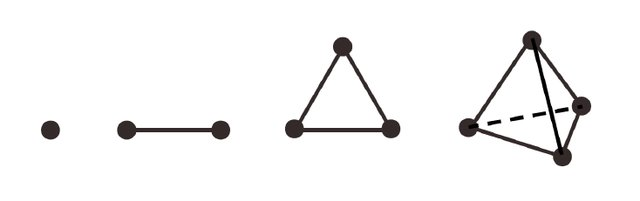
\includegraphics[width=.65\textwidth]{figures/simplices.jpg}};
	\end{tikzpicture}
\end{figure}

\begin{definition}
	A \textbf{singular $r$-simplex in a topological space $M$} is a continuous map $\sigma^r : U \to M$ where $U$ is an open neighbourhood of a $\Delta^r \subseteq \R^r$.
\end{definition}

By abuse of terminology, often we'll call $r$-simplex in $M$ the image of $\sigma^r$.

\begin{construction}
	Using the family of singular $r$-simplices in a topological space $M$ as generators, we can build a free $R$-module $C_r(M; R)$ for all commutative rings $R$ (usually $R$ is $\Z$, $\Q$, $\R$ or $\C$.). An element of such module is called an \textbf{$r$-chain} and it is a formal sum of $r$-simplices in $M$ with coefficients taken from $R$.
\end{construction}

\begin{definition}
	The \textbf{boundary} of an $r$-simplex $\sigma^r$ of $M$ is the $(r-1)$-chain $\partial \sigma^r$ defined as
	\begin{eqalign}
		\partial \sigma^r := \sum_{k=0}^r (-1)^k [P_0, \ldots, \hat{P_k}, \ldots, P_r]
	\end{eqalign}
	where $\hat{-}$ means we are skipping the term underneath.
\end{definition}

The terms, without sign, appearing in the summation defining $\partial \sigma^r$ are called \textbf{faces} of the simplex. Thus the boundary of a simplex is the alternating sum of its faces.

By $R$-linear extension, the boundary construction induces a (family of) map(s) $\partial : C_r(M; R) \to C_{r-1}(M; R)$, called the \textbf{boundary map(s)}.

\begin{lemma}
	The boundary maps are boundary maps in the sense of homological algebra, i.e.
	\begin{eqalign}
		\partial_{r-1} \partial_r = 0
	\end{eqalign}
\end{lemma}
\begin{proof}
	For conciseness sake, define
	\begin{eqalign}
		[\hat{h}, \hat{k}] = [p_0, \ldots, \hat{p_h}, \ldots, \hat{p_k}, \ldots, p_r].
	\end{eqalign}
	Notice to show the claim it suffices to prove it for a single, arbitrary $r$-simplex, as they generate $C_r(M; R)$. Then it is just a matter of computation. We just need to be careful substituting the second $\partial$ as indices for it have to be properly shifted:
	\begin{eqalign}
		\partial (\partial [p_0, \ldots, p_r]) &= \sum_{k=0}^r (-1)^k \partial [\hat{k}]\\
		&=\sum_{k=0}^r (-1)^k \left( \sum_{h=0}^{k-1} (-1)^h [\hat{h}, \hat{k}] + \sum_{h=k+1}^r (-1)^{h-1} [\hat{k}, \hat{h}] \right)\\
		&= \sum_{0 \leq h < k \leq r} (-1)^{k+h} [\hat{h}, \hat{k}] - \sum_{0 \leq k < h \leq r} (-1)^{k+h} [\hat{h}, \hat{k}] = 0,
	\end{eqalign}
	The very last equality is proven by swapping the indices of one summation (both will do) -- as its apparent this operation doesn't add nor remove any term; and simply noticing we then get two equal things subtracted, hence zero.
\end{proof}

Chains $\sigma^r \in C_r$ such that $\partial \sigma^r = 0$ are called \textbf{cycles} ($\sigma^r \in Z^r(M; R) = \ker \partial_r$ in symbols), while when $\partial \delta = \sigma$ for some $\delta \in C_{r+1}$ we speak of \textbf{boundaries} (in symbols $\sigma^r \in B^r(M; R) = \im \partial_{r+1}$).

\begin{definition}
	The \textbf{$r$-th singular homology of $M$ with coefficients in $R$} is
	\begin{eqalign}
		H_r(M; R) := \ker \partial_r / \im \partial_{r+1} = Z^r(M; R) / B^r(M; R)
	\end{eqalign}
\end{definition}

\subsection{de Rham's Theorem}
\label{subsec:de_rham}
Unlike de Rham cohomology, singular homology is a topological construction. On the other hand, on a smooth manifold $M$ we could have defined a ``smooth version'' by asking the maps $\sigma^r : U \to M$ to be not just continuous but smooth. Eventually, the two constructions turn out to be equivalent so we don't distinguish them in the following notation, but it's important to point out this is where the bridge between topological and \emph{differential} structure is crossed.

The aim of this section is then to prove smooth singular homology can be computed as well using de Rham cohomology, thus an easier and more tame machinery. To link the two, we'll use the natural pairing of differential forms and smooth simplicial chains given by integration:
\begin{eqalign}
	(-,-) : C^r(M; \R) \times \Omega^r(M) &\longto \R\\
	(\sum_{i=1}^n \alpha_n \sigma^r_n, \omega) &\longmapsto \int_C \omega := \sum_{i=1}^n \alpha_n \int_{\sigma^r_n} \omega
\end{eqalign}
Notice we fixed $R=\R$ for the coefficients of the homology as to get reals out of the integral.

A classical result links homological properties of differential forms to those of smooth simplicial chains:

\begin{theorem}[Stokes]
\label{th:stokes}
	Let $\omega \in \Omega^r(M)$ and $C$ be a smooth $(r+1)$-chain. Then
	\begin{eqalign}
		\int_{\partial C} \omega = \int_C d\omega
	\end{eqalign}
\end{theorem}

\begin{lemma}
	The integral pairing passes to homology and cohomology, i.e. the pairing
	\begin{eqalign}
		[-, -] : H_r(M; \R) \times H^r_{dR}(M) \longto \R
	\end{eqalign}
	defined by
	\begin{eqalign}
		[\overline C, \overline \omega] = (C, \omega)
	\end{eqalign}
	is a well-defined bilinear form.
\end{lemma}
\begin{proof}
	Choose $C' \in C^{r+1}(M; \R)$ and $\omega' \in \Omega^{r-1}$, then
	\begin{eqalign}
		C + \partial C' \in \overline C, \quad \omega + d\omega' \in \overline \omega
	\end{eqalign}
	so that to show well-definedness we simply need to show the result does not depend on $C'$ and $\omega'$. Indeed, applying the extended definition of the integral, Stokes' Theorem and recalling $\partial C=0$ and $d\omega = 0$ by definition of (co)homology, we get:
	\begin{eqalign}
		[\overline C, \overline\omega] &= (C + \partial C', \omega + d\omega')\\
			&= \int_C \omega + \int_{\partial C'} \omega + \int_C d\omega' + \int_{\partial C'} d\omega'\\
			&= \int_C \omega + \int_{C'} d\omega + \int_{\partial C} \omega' + \int_{\partial^2 C'} \omega' = (C, \omega).
	\end{eqalign}
	Bilinearity is then evident.
\end{proof}

\begin{theorem}[de Rham]
\label{th:de_rham}
	The bilinear form $[-,-]$ defined above is non-degenerate, hence it induces an isomorphism
	\begin{eqalign}
		H_r(M; \R) \isoin{\Vec} H_{dR}^r(M)
	\end{eqalign}
\end{theorem}

\begin{theorem}[Poincarè's duality]
	Let $M$ be a \emph{compact} orientable manifold of dimension $m$. The map
	\begin{eqalign}
		\langle -, - \rangle : H_{dR}^r(M) \times H_{dR}^{m-r}(M) &\longto \R\\
		( \overline \omega, \overline \eta) &\longmapsto \int_M \omega \wedge \eta
	\end{eqalign}
	is a well-defined, non-degenerate bilinear form, implying $H_{dR}^r(M) \isoin\Vec H_{dR}^{m-r}(M)$.
\end{theorem}
\begin{proof}[Proof sketch]
	For a compact orientable manifold we can produce a triangulation of $M$, that is, an $m$-chain homeomorphic to $M$ itself. By compactness of $M$, the chain must be a cycle since $\partial M = 0$. However it can't be the boundary of anyhting bigger since it is of maximal dimension. Then by de Rham's again,
	\begin{eqalign}
		\int_{\Delta_m} \omega \wedge \eta \neq 0
	\end{eqalign}
	proving the theorem.
\end{proof}

\begin{definition}
	The \textbf{Euler characteristic} of $M$ is the alternating sum of the dimensions of the homology groups of $M$:
	\begin{eqalign}
		\chi_M = \sum_{n=0}^{\dim M} (-1)^n \dim H_n(M)
	\end{eqalign}
\end{definition}

\begin{corollary}
	Any odd-dimensional compact orientable smooth manifold has $\chi_M = 0$.
\end{corollary}
\begin{proof}
	By de Rham's Theorem and Poincarè's duality.
\end{proof}

\paragraph{Induced maps.} \label{par:ind_maps_on_de_rham} Singular homology and de Rham cohomology are actually a family of functors, in the sense that maps between manifolds induce also maps between their cohomology groups in a way that is well-behaved with respect to composition. Indeed, if $f:X \to Y$ is a smooth map, it also brings singular simplices on $X$ to singular simplices on $Y$:
\begin{diagram}
	\& \Delta^n \arrow{dl}{\sigma} \arrow[dashed]{dr}{f \circ \sigma}\\
	X \arrow{rr}{f} \& \& Y
\end{diagram}
thereby producing a morphism $f^* : H_n(X; R) \to H_n(Y; R)$. The same thing happens for cohomology groups, although with a different variancy, by using the pullback of forms (Construction~\ref{const:pullback}), so we get a morphism $f^\sharp : H_{dR}^n(Y) \to H_{dR}^n(X)$.

When $f_0, f_1 : M_1 \to M_2$ are smooth maps, to say they're \textbf{smoothly homotopic} means there is a ``smooth map interpolating between the two'', i.e. a smooth map
\begin{eqalign}
	h: M_1 \times [0,1] \to M_2,\ (p,t) \mapsto h_t(p)
\end{eqalign}
such that
\begin{eqalign}
	h_0 = f_0, \quad h_1 = f_1.
\end{eqalign}
Then it can be shown that \textbf{the whenever $f_0$ and $f_1$ are homotopic, they induce the same homeomorphisms $f_0^\sharp$ and $f_1^\sharp$ on the de Rham cohomology groups}.

\section{Interior product}
\begin{definition}[Interior product]
	Let $X \in \fields(M)$. The \textbf{interior product} with $X$ of a $(p+1)$-differential form $\omega$ is the unique $p$-differential form defined by
	\begin{eqalign}
		\ipr{X} \omega (X_1, \ldots, X_p) = \omega(X, X_1, \ldots, X_p), \quad \forall X_1, \ldots, X_p \in \fields(M).
	\end{eqalign}
\end{definition}

\begin{property}
	Let $X \in \fields(M)$, $\omega \in \Omega^p(M)$ and $\eta \in \Omega^q(M)$. Then the following hold:
	\begin{enumerate}
		\item $\ipr{X}$ is a boundary map:
		\begin{eqalign}
			\ipr{X}^2 = 0.
		\end{eqalign}
		\item $\ipr{X}$ is an \textbf{graded antiderivation}:
		\begin{eqalign}
		\label{eq:int_prod_graded_antid}
			\ipr{X}(\omega \wedge \eta) = (\ipr{X} \omega) \wedge \eta + (-1)^p \omega \wedge (\ipr{X} \eta).
		\end{eqalign}
		\item $\ipr{X}$ commutes with the Lie derivative along $X$:
		\begin{eqalign}
			\Lie{X} \ipr{X} = \ipr{X} \Lie{X}.
		\end{eqalign}
		\item Cartan's magic formula:
		\begin{eqalign}
		\label{eq:cartan_magic_formula}
			\Lie{X} \omega = d(\ipr{X} \omega) + \ipr{X} (d \omega).
		\end{eqalign}
	\end{enumerate}
\end{property}

\subsection{Integration}
\begin{definition}
	A \textbf{volume form} on the $n$-dimensional manifold $M$ is given by an $n$-differential form
\end{definition}

\end{document}